\newpage
\setcounter{section}{2}
\setcounter{subsection}{0}
\Section{Dataset 2: The Wine Quality}

In this Section, we will present the classification results of the first dataset that we used in our project, which is the UCI Wine Quality dataset \cite{wine_quality}.

The Wine Quality dataset contains data related to red and white variants of the Portuguese "Vinho Verde" wine. The dataset includes physicochemical input variables (e.g., acidity, sugar content, alcohol) and an output variable representing the wine quality. Detailed information about the wine can be found at \url{http://www.vinhoverde.pt/en/} or in the reference by Cortez et al. (2009). 

\subsubsection*{Dataset Characteristics}
\begin{itemize}
    \item \textbf{Type:} Multivariate
    \item \textbf{Subject Area:} Business
    \item \textbf{Associated Tasks:} Classification, Regression
    \item \textbf{Feature Type:} Real
    \item \textbf{Number of Instances:} 4898
    \item \textbf{Number of Features:} 11
    \item \textbf{Missing Values:} No
\end{itemize}

\subsubsection*{Dataset Insights}
\begin{itemize}
    \item \textbf{Data source:} The dataset is derived from physicochemical and sensory tests. No information is provided about grape types, wine brand, or pricing due to privacy and logistical constraints.
    \item \textbf{Task type:} The dataset can be used for both classification and regression tasks. In this project, we focus on the classification task by grouping wine quality into broader categories.
    \item \textbf{Class imbalance:} The dataset is imbalanced, with more samples representing average-quality wines than excellent or poor-quality ones.
    \item \textbf{Feature selection:} Some input variables may not be relevant, making this dataset suitable for testing feature selection methods.
\end{itemize}

\subsubsection*{Feature Description}
\begin{itemize}
    \item \textbf{Input Variables:}
    \begin{enumerate}
        \item Fixed acidity
        \item Volatile acidity
        \item Citric acid
        \item Residual sugar
        \item Chlorides
        \item Free sulfur dioxide
        \item Total sulfur dioxide
        \item Density
        \item pH
        \item Sulphates
        \item Alcohol
    \end{enumerate}
    \item \textbf{Output Variable:}
    \begin{itemize}
        \item Quality: A score between 0 and 10, categorized into three broader groups for analysis:
        \begin{enumerate}
            \item Low quality: Classes 0-4
            \item Standard quality: Classes 5-6
            \item High quality: Classes 7-10
        \end{enumerate}
    \end{itemize}
\end{itemize}

\subsection{Data preparation}

\subsubsection{Import the dataset}

The \href{https://archive.ics.uci.edu/}{UC Irvine Machine Learning Repository} allows for direct dataset import in Python using the \texttt{ucimlrepo} package. The package is included in the \texttt{requirements.txt} file. The following code demonstrates how to import the Wine Quality (id = 186) dataset using the \texttt{fetch\_ucirepo} function:

\lstset{style=code}
\begin{lstlisting}[language=Python]
from ucimlrepo import fetch_ucirepo 

breast_cancer_wisconsin_diagnostic = fetch_ucirepo(id=186) 
    
X = breast_cancer_wisconsin_diagnostic.data.features 
y = breast_cancer_wisconsin_diagnostic.data.targets 
\end{lstlisting}

\subsubsection{Splitting the dataset}

The dataset is split into training and testing sets using the \texttt{train\_test\_split} function from the \texttt{sklearn} library. 
The dataset is splitted into 4 sets of different test sizes: 60\%, 40\%, 20\%, and 10\% of the dataset in stratified fashion, using the random state of 22125 to ensure reproducibility.

\begin{figure}[H]
    \centering
    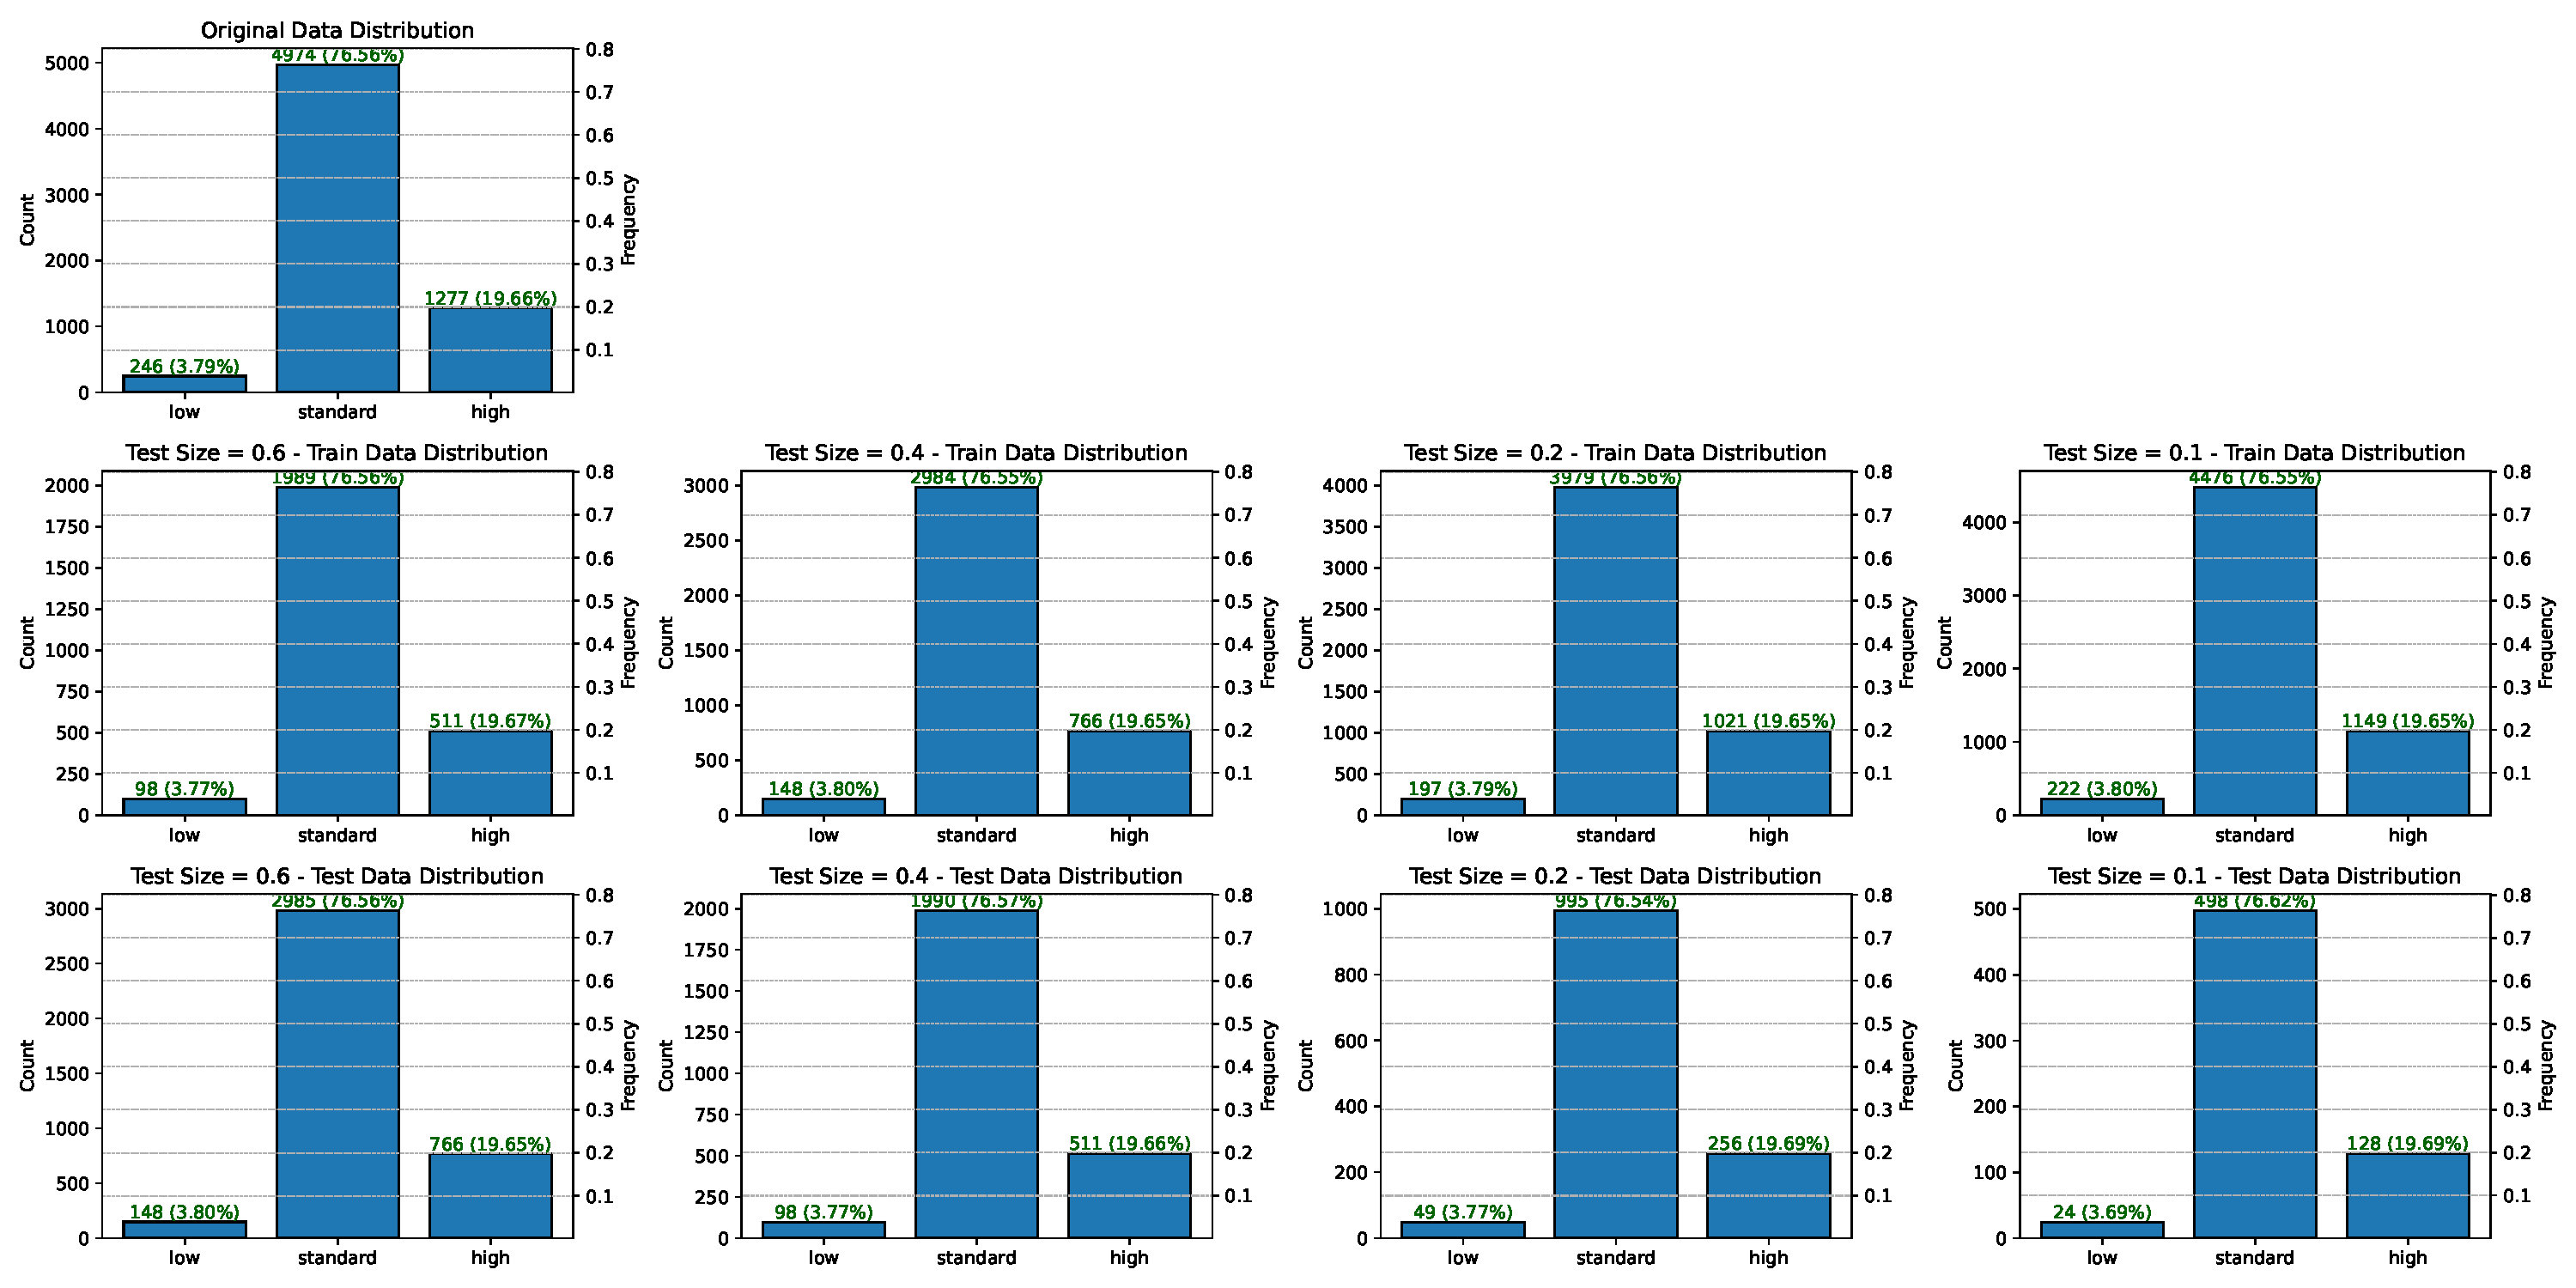
\includegraphics[width=\textwidth]{figures/wine_quality_split.pdf}
    \caption{Breast Cancer Wisconsin dataset split}
    \label{fig:wine_quality_split}
\end{figure}

As shown in figure \ref{fig:wine_quality_split}, the distribution of the target class is preserved in all splits.

\subsection{Decision Tree classifier implementation}

Decision Tree classifiers are implemented using the \texttt{DecisionTreeClassifier} class from the \texttt{sklearn} library. 
To ensure reproducibility, the random state is set to 22125. 
We use the Entropy (information gain) criterion to split the nodes and set the maximum depth of the tree to None to allow the tree to grow until all leaves are pure.

\begin{figure}[H]
    \centering
    \includegraphics[width=\textwidth]{figures/breast_cancer_wisconsin_decision_trees.pdf}
    \caption{Wine Quality dataset Decision Trees with different test sizes}
    \label{fig:wine_quality_decision_trees}
\end{figure}

The Decision Trees are visualized in figure \ref{fig:wine_quality_decision_trees}. 
The depths of the trees for the test sizes 60\%, 40\%, 20\%, and 10\% are 24, 23, 22, and 26 respectively. This indicates that the model complexity does not consistently increase or decrease with the test size.

The first node of the Decision Tree agrees on the feature \texttt{alcohol} to split the dataset for all test sizes. This feature is likely the most discriminative for classifying the wine quality in the dataset.

The first node's entropy is approximately 0.935 in all Decision Trees, indicating that the first split is not very informative. However, the Decision Tree classifier effectively splits the dataset into pure leaves with high information gain.

\subsection{Performance evaluation}

\subsubsection{Classification report}

The classification report provides a comprehensive evaluation of the Decision Tree classifier's performance using the \texttt{classification\_report} function from the \texttt{sklearn.metrics} module. The report includes the following metrics:
\begin{itemize}
    \item \textbf{Precision:} The ratio of true positive samples to the sum of true positive and false positive samples.
    \item \textbf{Recall:} The ratio of true positive samples to the sum of true positive and false negative samples.
    \item \textbf{F1-score:} The harmonic mean of precision and recall.
    \item \textbf{Support:} The number of samples in each class.
\end{itemize}

\textbf{Classification Report for Test Size = 0.6}

\begin{tabular}{lcccccc}
\hline
 & \textbf{Precision} & \textbf{Recall} & \textbf{F1-score} & \textbf{Support} \\
\hline
Low & 0.18 & 0.16 & 0.17 & 148 \\
Standard & 0.85 & 0.85 & 0.85 & 2985 \\
High & 0.53 & 0.55 & 0.54 & 766 \\
\hline
\textbf{Accuracy} & & & 0.76 & 3899 \\
\textbf{Macro avg} & 0.52 & 0.52 & 0.52 & 3899 \\
\textbf{Weighted avg} & 0.76 & 0.76 & 0.76 & 3899 \\
\hline
\end{tabular}

\vspace{2em}

\textbf{Classification Report for Test Size = 0.4}

\begin{tabular}{lcccccc}
\hline
 & \textbf{Precision} & \textbf{Recall} & \textbf{F1-score} & \textbf{Support} \\
\hline
Low & 0.15 & 0.16 & 0.16 & 98 \\
Standard & 0.85 & 0.86 & 0.85 & 1990 \\
High & 0.57 & 0.55 & 0.56 & 511 \\
\hline
\textbf{Accuracy} & & & 0.77 & 2599 \\
\textbf{Macro avg} & 0.52 & 0.52 & 0.52 & 2599 \\
\textbf{Weighted avg} & 0.77 & 0.77 & 0.77 & 2599 \\
\hline
\end{tabular}

\vspace{2em}

\textbf{Classification Report for Test Size = 0.2}

\begin{tabular}{lcccccc}
\hline
 & \textbf{Precision} & \textbf{Recall} & \textbf{F1-score} & \textbf{Support} \\
\hline
Low & 0.19 & 0.24 & 0.22 & 49 \\
Standard & 0.85 & 0.86 & 0.86 & 995 \\
High & 0.58 & 0.54 & 0.56 & 256 \\
\hline
\textbf{Accuracy} & & & 0.77 & 1300 \\
\textbf{Macro avg} & 0.54 & 0.55 & 0.54 & 1300 \\
\textbf{Weighted avg} & 0.77 & 0.77 & 0.77 & 1300 \\
\hline
\end{tabular}

\vspace{200em}

\textbf{Classification Report for Test Size = 0.1}

\begin{tabular}{lcccccc}
\hline
 & \textbf{Precision} & \textbf{Recall} & \textbf{F1-score} & \textbf{Support} \\
\hline
Low & 0.32 & 0.33 & 0.33 & 24 \\
Standard & 0.86 & 0.86 & 0.86 & 498 \\
High & 0.56 & 0.56 & 0.56 & 128 \\
\hline
\textbf{Accuracy} & & & 0.78 & 650 \\
\textbf{Macro avg} & 0.58 & 0.59 & 0.58 & 650 \\
\textbf{Weighted avg} & 0.78 & 0.78 & 0.78 & 650 \\
\hline
\end{tabular}

The classification reports show that the Decision Tree classifier achieves high precision, recall, and F1-score for the standard quality class. The classifier performs poorly on the low-quality class due to the class imbalance in the dataset. The high-quality class has moderate performance, with precision, recall, and F1-score around 0.5-0.6.

\subsubsection{Confusion matrix}

The confusion matrix provides a visual representation of the Decision Tree classifier's performance using the \texttt{confusion\_matrix} function from the \texttt{sklearn.metrics} module. The matrix shows the number of true positive, false positive, true negative, and false negative samples for each class.

\begin{figure}[H]
    \centering
    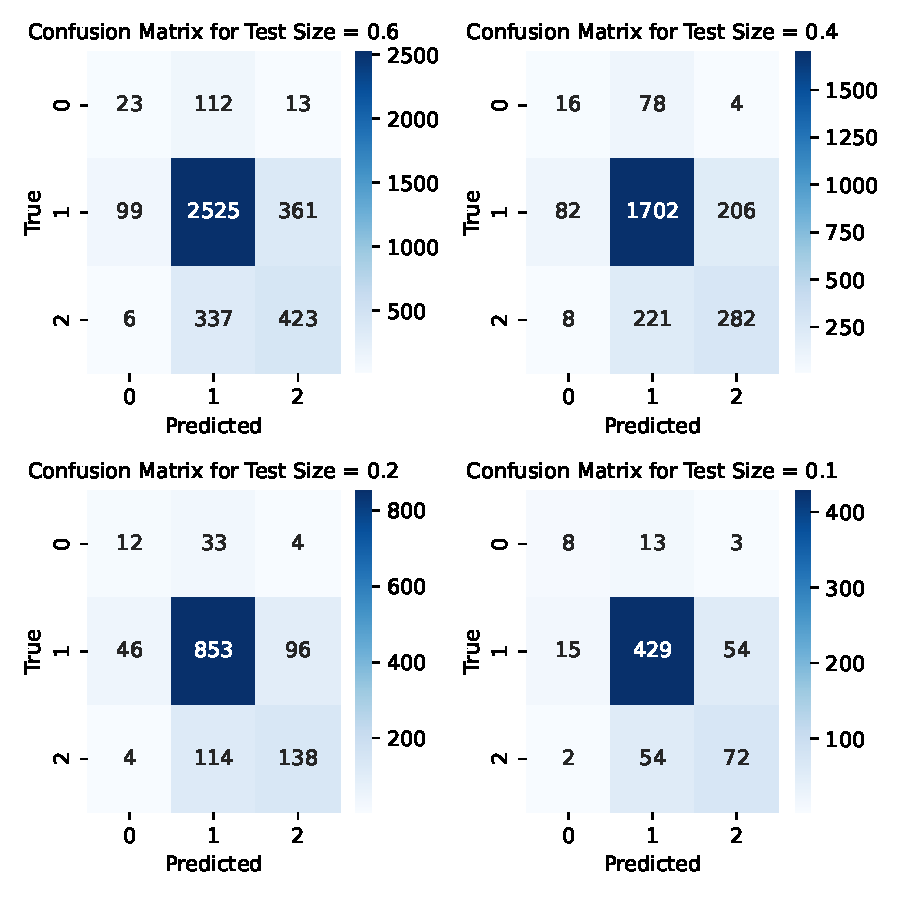
\includegraphics[width=.7\textwidth]{figures/wine_quality_confusion_matrices.pdf}
    \caption{Wine Quality dataset Confusion Matrices with different test sizes}
    \label{fig:wine_quality_confusion_matrices}
\end{figure}
% Confusion Matrix for Test Size = 0.6:
% [[  23  112   13]
%  [  99 2525  361]
%  [   6  337  423]]
% Confusion Matrix for Test Size = 0.4:
% [[  16   78    4]
%  [  82 1702  206]
%  [   8  221  282]]
% Confusion Matrix for Test Size = 0.2:
% [[ 12  33   4]
%  [ 46 853  96]
%  [  4 114 138]]
% Confusion Matrix for Test Size = 0.1:
% [[  8  13   3]
%  [ 15 429  54]
%  [  2  54  72]]

The confusion matrices in figure \ref{fig:wine_quality_confusion_matrices} show that the Decision Tree classifier performs well on the standard quality class but struggles with the low and high-quality classes. The classifier misclassifies many low-quality samples as standard quality and high-quality samples as standard quality. This behavior is expected due to the class imbalance in the dataset.

\subsection{Depth vs Accuracy evaluation}

The Decision Tree classifier's performance is evaluated by varying the maximum depth of the tree. The accuracy of the classifier is computed for different maximum depths using the \texttt{accuracy\_score} function from the \texttt{sklearn.metrics} module for the Decision Tree classifier with a test size of 20\%.

\begin{figure}[H]
    \centering
    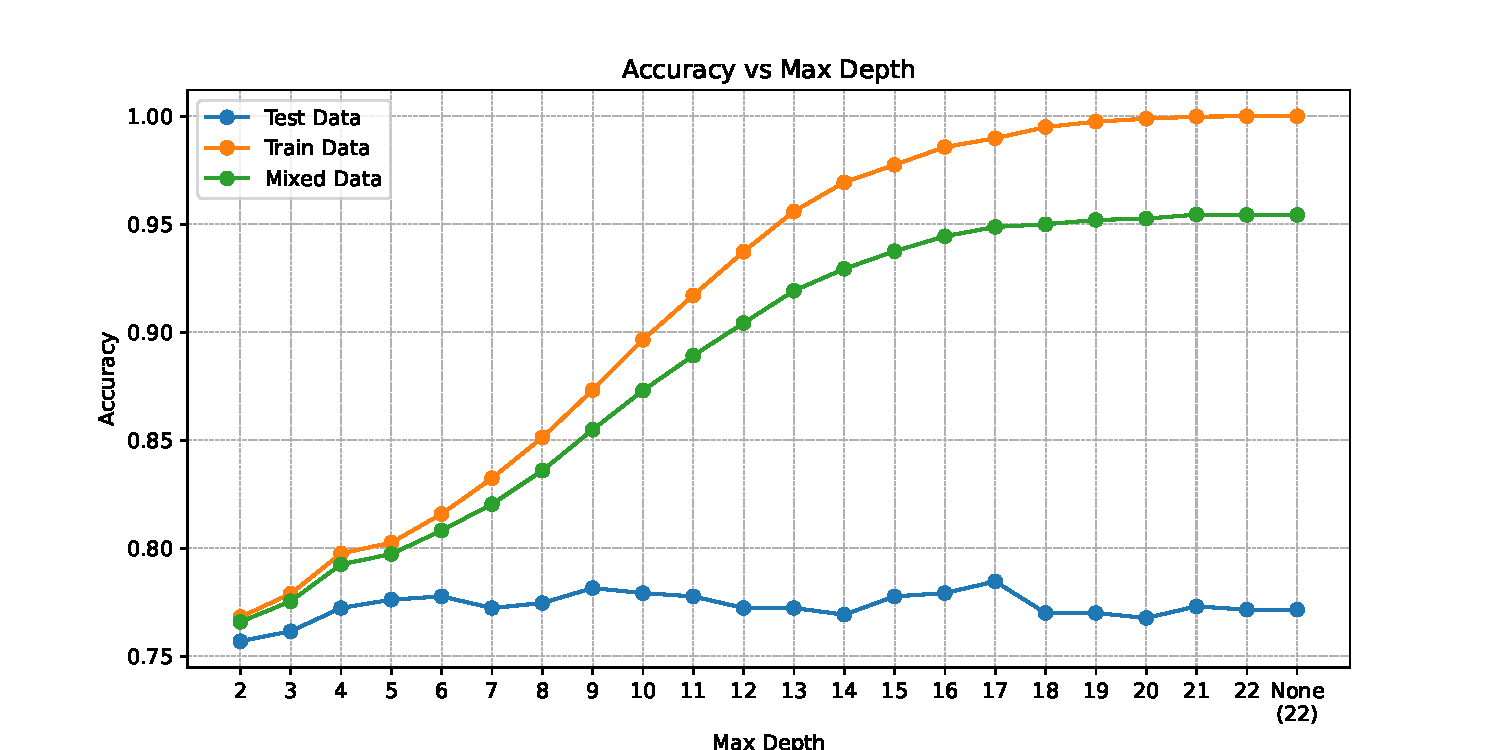
\includegraphics[width=\textwidth]{figures/wine_quality_accuracy_vs_max_depth.pdf}
    \caption{Breast Cancer Wisconsin dataset Depth vs Accuracy}
    \label{fig:wine_quality_accuracy_vs_max_depth}
\end{figure}

The plot in figure \ref{fig:wine_quality_accuracy_vs_max_depth} shows that the Decision Tree classifier achieves the highest accuracy on the test data when the maximum depth is around 17. The accuracy slightly fluctuates around 0.77 for all depths, indicating that the model's performance is relatively stable.

